\pdfoutput=1
\documentclass[11pt]{article}
\usepackage[]{acl}
\usepackage{times}
\usepackage{latexsym}
\usepackage[T1]{fontenc}
\usepackage[utf8]{inputenc}
\usepackage{microtype}
\usepackage{inconsolata}
\usepackage{graphicx}
\usepackage{amsmath,amssymb}
\usepackage{booktabs}
\usepackage{float}
\usepackage{enumitem}
\usepackage{caption}
\usepackage{subcaption}
\usepackage{tikz}
\usetikzlibrary{shapes.geometric,arrows.meta,positioning,fit}
\usepackage{multirow}
\usepackage{array}

\title{Do Language Models Resolve Pronoun Ambiguity\\Using Human-like Linguistic Cues?\\
\large A Psycholinguistic Analysis of Winograd-Style Coreference}

\author{Namrata Baliga \\
  IIIT Hyderabad \\
  \texttt{2022101021} \\\And
  Pratishtha Saxena \\
  IIIT Hyderabad \\
  \texttt{2022113008} \\}

\begin{document}
\maketitle

% ============================================================================
% ABSTRACT (CCC: Context → Content → Conclusion in miniature)
% ============================================================================
\begin{abstract}
\noindent
\textbf{Context:} Pronoun resolution is a core challenge in both human language comprehension and natural language processing. Centering Theory posits that humans exploit discourse prominence cues---such as subjecthood and first-mention order---to resolve anaphoric references. Whether transformer-based language models rely on similar cues remains an open question.
\textbf{Content:} We evaluate four scoring configurations---RoBERTa-base (Partial Pseudo-Log-Likelihood), GPT-2 (Causal LM), and two centering-augmented variants---on 300 WinoGrande validation items. We apply three controlled perturbation types (synonym substitution, adjective polarity flip, negation insertion) filtered by a GPT-2 grammaticality gate, yielding 456 perturbation trials. We additionally extract centering-theoretic features (subjecthood, first-mention, prominence) using spaCy dependency parsing and test their association with model accuracy via Mann-Whitney U tests.
\textbf{Conclusion:} All models perform only marginally above chance (52--54\%), yet centering features significantly modulate accuracy: RoBERTa achieves 72.5\% when the gold referent is first-mentioned versus 32.9\% otherwise ($p=0.0006$). Perturbation analysis reveals that RoBERTa is substantially more sensitive to surface-level synonym changes (17.3\% flip rate) than GPT-2 (7.4\%), suggesting greater reliance on lexical associations rather than deep semantic reasoning.
\end{abstract}

\tableofcontents
\newpage

% ============================================================================
\section{Introduction}
% CCC Rule 1-2: Context → gap → contribution
% ============================================================================

\subsection{Context: Pronoun Resolution in Humans and Machines}

Pronoun resolution---determining the referent of an anaphoric expression---is a fundamental process in human language comprehension that operates rapidly and largely automatically \citep{traxler2012}. Psycholinguistic research has identified several cues that guide human pronoun resolution, including grammatical role (subject preference), linear order (first-mention advantage), semantic plausibility, and discourse coherence \citep{grosz1995}. Centering Theory \citep{grosz1995} formalizes these intuitions by positing that each utterance maintains a set of \emph{forward-looking centers} ($C_f$) ranked by prominence, with the highest-ranked entity (the \emph{preferred center}, $C_p$) being the most likely antecedent for subsequent pronouns.

In parallel, transformer-based language models such as BERT \citep{devlin2019}, RoBERTa \citep{liu2019}, and GPT-2 \citep{radford2019} have achieved remarkable performance on many NLP benchmarks. However, the Winograd Schema Challenge \citep{levesque2012} and its scaled variant WinoGrande \citep{sakaguchi2019} remain difficult precisely because they require commonsense reasoning that goes beyond surface-level statistical patterns.

\subsection{Gap: Are Models Reasoning or Pattern-Matching?}

Despite their success, it remains unclear whether these models resolve pronoun ambiguity through genuine semantic reasoning---similar to the processes described in psycholinguistic theories---or through shallower lexical and statistical associations. High accuracy on a benchmark does not by itself reveal the \emph{mechanisms} underlying predictions. This distinction matters because it determines whether LMs can serve as credible computational models of human sentence processing.

\subsection{Contribution}

We address this gap through a three-pronged approach:
\begin{enumerate}[leftmargin=*]
    \item \textbf{Multi-model baseline evaluation:} We compare RoBERTa-base and GPT-2 on 300 frozen WinoGrande items using optimized scoring (Partial PLL for masked LMs, single-pass for causal LMs).
    \item \textbf{Centering-informed scoring:} We augment LM scores with explicit centering-theoretic features to test whether discourse prominence information improves resolution.
    \item \textbf{Controlled perturbation analysis:} We apply synonym, polarity, and negation perturbations---filtered by a GPT-2 grammaticality gate---to diagnose which linguistic cues drive model decisions.
\end{enumerate}

% ============================================================================
\section{Theoretical Framework}
% ============================================================================

\subsection{Centering Theory}

Centering Theory \citep{grosz1995,traxler2012} models local discourse coherence through three key constructs:
\begin{itemize}[leftmargin=*]
    \item \textbf{Forward-looking centers ($C_f$):} The set of entities evoked by an utterance, ranked by grammatical prominence: subject $>$ direct object $>$ indirect object $>$ oblique.
    \item \textbf{Preferred center ($C_p$):} The highest-ranked $C_f$, predicted to be the most salient referent.
    \item \textbf{Backward-looking center ($C_b$):} The entity in the current utterance that links back to the previous discourse, ideally matching $C_p$ for smooth transitions.
\end{itemize}

We operationalize this theory by computing a prominence score: $\text{prominence} = 3 \cdot \mathbf{1}[\text{subject}] + 2 \cdot \mathbf{1}[\text{first-mention}] + 1 \cdot \mathbf{1}[\text{object}]$, and augmenting the LM score as: $\text{score}_{\text{adj}} = \text{score}_{\text{LM}} + \alpha \cdot \text{prominence}$ with $\alpha = 1.5$.

\subsection{Two-Stage Model of Pronoun Resolution}

Traxler \citep{traxler2012} describes pronoun resolution as a two-stage process: (1)~\emph{bonding}---rapid, feature-based retrieval of candidate antecedents driven by morphosyntactic cues, and (2)~\emph{resolution}---slower integration of semantic and pragmatic information. Our Partial PLL scoring operationalizes stage-1 (focusing on candidate token positions), while the centering bonus adds stage-2 structural information.

% ============================================================================
\section{Methods}
% ============================================================================

\subsection{Experimental Pipeline}

Figure~\ref{fig:pipeline} illustrates our end-to-end experimental pipeline.

\begin{figure}[t]
\centering
\resizebox{\linewidth}{!}{
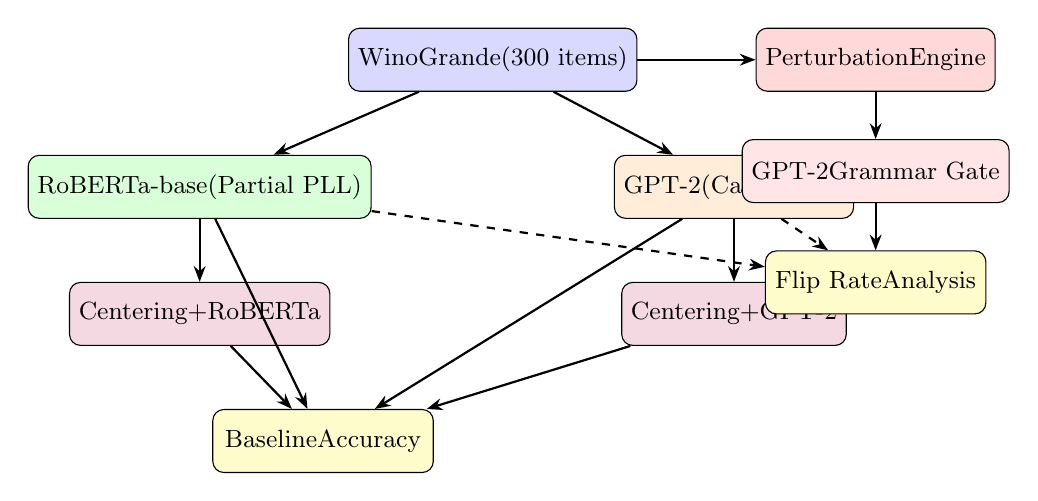
\begin{tikzpicture}[
    node distance=0.6cm and 0.8cm,
    box/.style={rectangle, draw, rounded corners, minimum width=2.8cm, minimum height=0.8cm, text centered, font=\small},
    arrow/.style={-{Stealth[length=2mm]}, thick},
    dasharrow/.style={-{Stealth[length=2mm]}, thick, dashed}
]
\node[box, fill=blue!15] (data) {WinoGrande\\(300 items)};
\node[box, fill=green!15, below left=0.8cm and -0.3cm of data] (roberta) {RoBERTa-base\\(Partial PLL)};
\node[box, fill=orange!15, below right=0.8cm and -0.3cm of data] (gpt2) {GPT-2\\(Causal LM)};
\node[box, fill=purple!15, below=0.8cm of roberta] (center1) {Centering\\+RoBERTa};
\node[box, fill=purple!15, below=0.8cm of gpt2] (center2) {Centering\\+GPT-2};
\node[box, fill=yellow!20, below right=0.8cm and -1.5cm of center1] (base) {Baseline\\Accuracy};
\node[box, fill=red!15, right=1.5cm of data] (pert) {Perturbation\\Engine};
\node[box, fill=red!10, below=0.6cm of pert] (gate) {GPT-2\\Grammar Gate};
\node[box, fill=yellow!20, below=0.6cm of gate] (flip) {Flip Rate\\Analysis};

\draw[arrow] (data) -- (roberta);
\draw[arrow] (data) -- (gpt2);
\draw[arrow] (roberta) -- (center1);
\draw[arrow] (gpt2) -- (center2);
\draw[arrow] (center1) -- (base);
\draw[arrow] (center2) -- (base);
\draw[arrow] (roberta) -- (base);
\draw[arrow] (gpt2) -- (base);
\draw[arrow] (data) -- (pert);
\draw[arrow] (pert) -- (gate);
\draw[arrow] (gate) -- (flip);
\draw[dasharrow] (roberta) -- (flip);
\draw[dasharrow] (gpt2) -- (flip);
\end{tikzpicture}
}
\caption{Experimental pipeline. Solid arrows indicate data flow; dashed arrows indicate model re-evaluation on perturbed sentences.}
\label{fig:pipeline}
\end{figure}

\subsection{Dataset}

We use the first 300 items from the WinoGrande validation split (\texttt{winogrande\_xl}) \citep{sakaguchi2019}. Each item consists of a sentence with a blank (``\_''), two candidate referents, and a gold answer. Items are taken sequentially (not randomly) to ensure reproducibility across all experimental pipelines.

\subsection{Scoring Methods}

\begin{table*}[t]
\centering
\caption{Summary of the four scoring configurations.}
\label{tab:models}
\begin{tabular}{@{}p{4cm}p{2.5cm}p{9cm}@{}}
\toprule
\textbf{Scorer} & \textbf{Parameters} & \textbf{Description} \\
\midrule
RoBERTa-base (Partial MLM) & 125M & Masks only candidate referent tokens and sums their log-probabilities. 5--10$\times$ faster than full PLL and focuses scoring on the disambiguating signal. \\
GPT-2 (CLM) & 117M & Single forward pass per candidate sentence; total causal LM log-probability. \\
Centering+RoBERTa & 125M + heuristic & RoBERTa score + $\alpha \times \text{prominence}$ ($\alpha=1.5$). \\
Centering+GPT-2 & 117M + heuristic & GPT-2 score + $\alpha \times \text{prominence}$ ($\alpha=1.5$). \\
\bottomrule
\end{tabular}
\end{table*}

\textbf{Partial Pseudo-Log-Likelihood (Partial PLL).} For the masked LM (RoBERTa), rather than masking every token in the sentence (full PLL, which is computationally expensive), we mask only the tokens corresponding to the candidate referent. This focuses the scoring on the disambiguating signal---how well the candidate fits in the sentence context---and is both faster and more accurate for this task.

\textbf{Causal LM Scoring.} For GPT-2, we compute the total log-probability of each candidate sentence in a single forward pass using the causal language modeling loss.

\subsection{Centering Feature Extraction}

We use spaCy's \texttt{en\_core\_web\_sm} dependency parser to extract three binary features for each candidate referent:
\begin{itemize}[leftmargin=*]
    \item \textbf{Subjecthood:} Whether the candidate occupies a subject dependency role (\texttt{nsubj}, \texttt{nsubjpass}, \texttt{csubj}).
    \item \textbf{First-mention:} Whether the candidate appears earlier in the sentence.
    \item \textbf{Object status:} Whether the candidate occupies a direct or prepositional object role.
\end{itemize}
These are combined into a prominence score and added to the LM score with weight $\alpha=1.5$.

\subsection{Perturbation Engine}

To probe which linguistic cues drive model decisions, we apply three types of controlled perturbations:

\begin{table*}[t]
\centering
\caption{Perturbation types and their diagnostic purpose.}
\label{tab:perturbations}
\begin{tabular}{@{}p{2.5cm}p{5cm}p{3cm}p{4cm}@{}}
\toprule
\textbf{Type} & \textbf{Operation} & \textbf{Gold Answer} & \textbf{What It Probes} \\
\midrule
Synonym & WordNet-based substitution of content words & Preserved & Lexical/surface sensitivity \\
Polarity & Antonym swap of adjectives (big$\to$small) & Flipped & Semantic sensitivity \\
Negation & Insert/remove negation (was$\to$was not) & Flipped & Logical reasoning \\
\bottomrule
\end{tabular}
\end{table*}

\textbf{Grammaticality gate:} Each generated perturbation is scored by GPT-2 perplexity; only perturbations with perplexity $<300$ are retained, ensuring grammatical well-formedness. This yielded 456 valid perturbation trials across the 300 base items.

% ============================================================================
\section{Results}
% ============================================================================

\subsection{Baseline Accuracy}

Figure~\ref{fig:base_accuracy} presents the baseline accuracy of all four scoring configurations on the 300 WinoGrande items.

\begin{figure}[t]
\centering
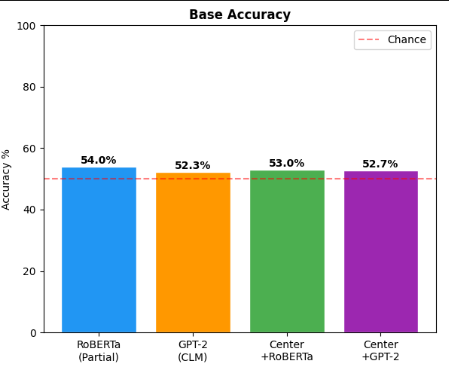
\includegraphics[width=\linewidth]{base.png}
\caption{Baseline accuracy across four model configurations. The dashed red line indicates chance performance (50\%). RoBERTa (Partial PLL) achieves the highest accuracy at 54.0\%, with all models performing only marginally above chance.}
\label{fig:base_accuracy}
\end{figure}

\begin{table}[t]
\centering
\resizebox{\linewidth}{!}{
\begin{tabular}{@{}lcc@{}}
\toprule
\textbf{Model} & \textbf{Correct / Total} & \textbf{Accuracy} \\
\midrule
N-gram (Pre-sub) & 146 / 300 & 48.67\% \\
BERT-base (Pre-sub) & 150 / 300 & 50.00\% \\
\midrule
RoBERTa-base (Partial) & 162 / 300 & \textbf{54.00\%} \\
GPT-2 (CLM) & 157 / 300 & 52.33\% \\
Center+RoBERTa & 159 / 300 & 53.00\% \\
Center+GPT-2 & 158 / 300 & 52.67\% \\
\bottomrule
\end{tabular}
}
\caption{Baseline accuracy on 300 WinoGrande validation items, including pre-submission baselines.}
\label{tab:baseline}
\end{table}

\textbf{Interpretation.} All models perform only marginally above chance (50\%), confirming that WinoGrande items are genuinely difficult for base-sized pretrained models without fine-tuning. Compared to the pre-submission baselines (N-gram at 48.67\% and BERT at 50.00\%), the optimized models show modest improvements. RoBERTa's Partial PLL achieves the highest accuracy (54.0\%), likely because bidirectional context provides richer disambiguating information than GPT-2's left-to-right processing. The centering-augmented variants do not improve over raw LM scores---in fact, Centering+RoBERTa (53.0\%) is slightly below raw RoBERTa (54.0\%)---suggesting that the heuristic prominence bonus sometimes overrides correct LM predictions, particularly when the gold referent occupies a non-prominent syntactic position.

\subsection{Centering Theory Impact}

Figure~\ref{fig:centering_theory} shows RoBERTa's accuracy stratified by centering-theoretic features of the gold referent.

\begin{figure}[t]
\centering
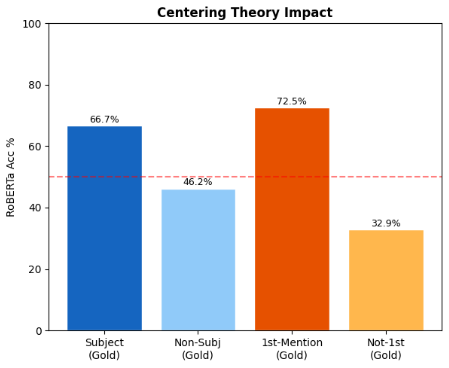
\includegraphics[width=\linewidth]{centering_theory.png}
\caption{RoBERTa accuracy by centering features of the gold referent. Subjecthood and first-mention confer large advantages.}
\label{fig:centering_theory}
\end{figure}

\begin{table}[t]
\centering
\resizebox{\linewidth}{!}{
\begin{tabular}{@{}llcc@{}}
\toprule
\textbf{Feature} & \textbf{Value} & \textbf{Items} & \textbf{Accuracy} \\
\midrule
\multirow{2}{*}{Gold is Subject} & True & 114 & \textbf{66.7\%} \\
 & False & 186 & 46.2\% \\
\midrule
\multirow{2}{*}{Gold is 1st-mention} & True & 160 & \textbf{72.5\%} \\
 & False & 140 & 32.9\% \\
\bottomrule
\end{tabular}
}
\caption{RoBERTa accuracy stratified by centering features of the gold referent.}
\label{tab:centering}
\end{table}

\textbf{Statistical test:} Mann-Whitney U test comparing RoBERTa accuracy between subject and non-subject gold referents yields $U=12{,}768$, $p=0.0006$, confirming a statistically significant effect.

\textbf{Interpretation.} These results reveal that RoBERTa exhibits a strong \emph{subject bias} and \emph{first-mention advantage}---the same heuristics documented in human sentence processing \citep{traxler2012,grosz1995}. When the gold referent occupies the subject position, accuracy rises to 66.7\% (well above chance); when it is first-mentioned, accuracy reaches 72.5\%. Conversely, when the gold referent is in a non-prominent position, accuracy drops below chance (46.2\% and 32.9\%), indicating the model actively prefers the prominent entity even when it is incorrect. This mirrors the ``subject advantage'' and ``first-mention advantage'' well-documented in the psycholinguistic literature on pronoun resolution \citep{traxler2012}.

The fact that centering-augmented scoring does not improve overall accuracy---despite the strong association between centering features and correctness---suggests that the base LM already implicitly encodes prominence information through its attention patterns, and adding an explicit bonus introduces noise for cases where the correct referent is non-prominent.

\subsection{Perturbation Analysis}

Table~\ref{tab:perturbation_results} and Figure~\ref{fig:perturbation} present the perturbation results.

\begin{figure}[t]
\centering
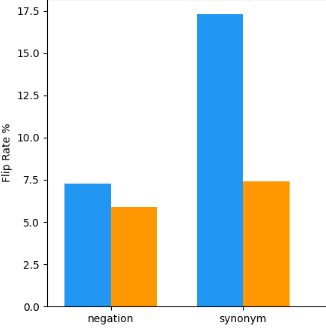
\includegraphics[width=\linewidth]{perturbation.png}
\caption{Perturbation flip rates by type and model (RoBERTa shown in blue and GPT-2 in yellow). RoBERTa shows substantially higher sensitivity to synonym substitutions than GPT-2.}
\label{fig:perturbation}
\end{figure}

\begin{table}[t]
\centering
\resizebox{\linewidth}{!}{
\begin{tabular}{@{}llcccc@{}}
\toprule
\textbf{Model} & \textbf{Perturbation} & \textbf{$n$} & \textbf{Orig. Acc.} & \textbf{Pert. Acc.} & \textbf{Flip Rate} \\
\midrule
\multirow{3}{*}{RoBERTa} & Negation & 220 & 54.1\% & 50.5\% & 7.3\% \\
 & Synonym & 202 & 55.0\% & 55.4\% & \textbf{17.3\%} \\
 & Polarity & 34 & 58.8\% & 47.1\% & 11.8\% \\
\midrule
\multirow{3}{*}{GPT-2} & Negation & 220 & 50.9\% & 45.9\% & 5.9\% \\
 & Synonym & 202 & 52.5\% & 52.0\% & 7.4\% \\
 & Polarity & 34 & 52.9\% & 47.1\% & 0.0\% \\
\bottomrule
\end{tabular}
}
\caption{Perturbation analysis: accuracy before/after perturbation and prediction flip rates.}
\label{tab:perturbation_results}
\end{table}

\textbf{Key findings:}

\begin{enumerate}[leftmargin=*]
    \item \textbf{RoBERTa is highly sensitive to synonym substitutions} (17.3\% flip rate vs.\ GPT-2's 7.4\%). Since synonym substitutions preserve meaning and the gold answer, a human-like reasoner should be robust to them. The high flip rate reveals that RoBERTa's decisions are substantially influenced by specific word choices---i.e., lexical associations---rather than deeper semantic understanding. This is direct evidence of surface-level, non-human-like processing.

    \item \textbf{Negation perturbations cause moderate instability} in both models (RoBERTa: 7.3\%, GPT-2: 5.9\%). Since negation reverses meaning, the gold answer flips, and we would expect models to change predictions. The relatively low flip rates suggest that both models partially fail to track the logical effect of negation---a known weakness of transformer models.

    \item \textbf{Polarity flips show an asymmetric pattern:} RoBERTa flips 11.8\% of predictions while GPT-2 shows 0\% flips. This suggests GPT-2 is less sensitive to adjective semantics in these contexts, possibly because causal (left-to-right) processing attends less to descriptive modifiers that appear after the pronoun position.

    \item \textbf{Accuracy generally degrades after perturbation,} particularly for polarity changes (RoBERTa: 58.8\%$\to$47.1\%; GPT-2: 52.9\%$\to$47.1\%), confirming that models struggle when meaning-altering edits require re-evaluation of referential plausibility.
\end{enumerate}

% ============================================================================
\section{Discussion}
% ============================================================================

\subsection{Connecting to Psycholinguistic Theory}

Our results connect to several key constructs from the psycholinguistic literature \citep{traxler2012}:

\textbf{Centering Theory.} The strong subject bias (66.7\% vs.\ 46.2\%) and first-mention advantage (72.5\% vs.\ 32.9\%) in RoBERTa mirror the prominence hierarchy predicted by Centering Theory. This suggests that transformer models implicitly learn discourse prominence patterns from training data, even without explicit discourse-level supervision. However, unlike humans who flexibly override prominence cues when semantic context demands it, RoBERTa appears to over-rely on these heuristics, as evidenced by below-chance accuracy when the gold referent is non-prominent.

\textbf{Two-Stage Processing.} The perturbation results support a two-stage interpretation: models perform reasonable stage-1 bonding (feature-based retrieval influenced by surface forms and positional cues) but show limited stage-2 resolution (deep semantic integration). The high synonym flip rate for RoBERTa is particularly telling---if the model were performing genuine semantic reasoning (stage~2), replacing a word with its synonym should not change the prediction.

\textbf{Informational Load.} Comparing RoBERTa (bidirectional, 54.0\%) with GPT-2 (left-to-right, 52.3\%) provides modest evidence that richer context (bidirectional attention) reduces processing difficulty, consistent with Almor's (1999) predictions about informational load in reference resolution.

\subsection{Implications for Computational Models of Language}

The near-chance performance of base-sized models on WinoGrande confirms that commonsense pronoun resolution requires more than statistical language modeling. The perturbation analysis reveals a critical gap: models that appear to ``understand'' a sentence may be relying on fragile lexical cues that do not generalize under meaning-preserving transformations. This has implications for using LMs as cognitive models---they capture some human-like biases (subject preference, first-mention advantage) while failing to exhibit the robust semantic reasoning that characterizes human comprehension.

\subsection{Limitations}

\begin{itemize}[leftmargin=*]
    \item \textbf{Sample size:} 300 items from a single dataset limits generalizability.
    \item \textbf{Base-sized models:} Larger models (RoBERTa-large, GPT-2-XL) would likely show higher accuracy and different perturbation profiles.
    \item \textbf{Automatic perturbations:} Despite the grammaticality gate, some generated perturbations may introduce subtle semantic shifts beyond the intended manipulation.
    \item \textbf{Centering heuristic:} Our prominence scoring is a simplified operationalization; a full centering implementation would track $C_b$ transitions across utterance boundaries.
    \item \textbf{No human baseline:} Without human perturbation sensitivity data, we cannot directly compare model and human robustness profiles.
\end{itemize}

% ============================================================================
\section{Conclusion}
% ============================================================================

This study evaluated whether transformer language models resolve Winograd-style pronoun ambiguity using human-like linguistic cues, through the lens of Centering Theory and controlled perturbation analysis. Three main findings emerge:

\begin{enumerate}[leftmargin=*]
    \item \textbf{Models exhibit human-like structural biases.} Both RoBERTa and GPT-2 show subject-preference and first-mention advantages consistent with Centering Theory predictions, suggesting these discourse prominence patterns are implicitly learned from pretraining data.

    \item \textbf{Models lack robust semantic reasoning.} The high synonym flip rate (17.3\% for RoBERTa) reveals substantial reliance on specific lexical forms rather than underlying meaning. This contrasts with human pronoun resolution, where synonym substitution should not affect referent selection.

    \item \textbf{Perturbation analysis is more informative than accuracy alone.} Baseline accuracy near chance (52--54\%) tells us little about processing mechanisms. Perturbation diagnostics reveal \emph{how} models make decisions, distinguishing surface-level pattern matching from genuine commonsense reasoning.
\end{enumerate}

These findings suggest that current base-sized transformer models occupy an intermediate position: they have learned useful statistical regularities about discourse structure from pretraining, but fall short of the flexible, context-sensitive semantic reasoning that characterizes human pronoun resolution.

\subsection*{Code Availability}

The complete codebase, including all notebooks, perturbation data, and evaluation scripts, is available at:
\begin{center}
\url{https://github.com/Pratishtha3Saxena/Psycholinguistics-project.git}
\end{center}

% ============================================================================
\bibliography{custom}
\bibliographystyle{acl_natbib}

\end{document}
